\chapter{Технологический раздел}
В данном разделе приведены выбор средств реализации, реализация функции на стороне БД, реализация сущностей и ограничений целостности, описание интерфейса доступа к БД и описание тестов.

\section{Выбор средств реализации}
В качестве языка программирования для разработки ПО был выбран язык С\#, потому что средствами этого языка можно реализовать все требуемые возможности \cite{src_cs}.

В качестве СУБД выбран PostgreSQL, поскольку в нем поддерживаются принципы ACID и стандарты SQL, а также он обладает высокой производительностью \cite{src_pg}.

Для работы с СУБД выбрана библиотека Npgsql, поскольку она полностью поддерживает работу с PostgreSQL из кода C\# \cite{src_npgsql}.

Для реализации пользовательского интерфейса ПО был выбран фреймворк ASP.NET. Данный фреймворк предоставляет необходимые инструменты для создания пользовательского WEB-интерфейса \cite{src_asp}.

В качестве среды разработки выбрана Visual Studio, поскольку эта среда хорошо подходит для разработки приложений на платформе .NET~(C\#) \cite{src_vscode}.

\section{Реализация функции на стороне БД}
На листинге \ref{lst_function} приведена реализация функция на стороне БД, возвращающая значение атрибута Id для добавляемого в таблицу объекта.
\newpage
\begin{lstlisting}[label=lst_function,caption=\raggedright{Реализация функции на стороне БД}]
CREATE OR REPLACE FUNCTION next_id(tname text)
RETURNS INT
AS $$
DECLARE ret INT;
BEGIN
	EXECUTE 'SELECT max(id) + 1 FROM ' || tname INTO ret;
	IF ret IS NULL THEN
		ret = 1;
	END IF;
	RETURN ret;
END
$$
LANGUAGE plpgsql;
\end{lstlisting}

\section{Реализация сущностей и ограничений целостности}
На листингах \ref{lst_db1}--\ref{lst_db3} приведена реализация сущностей в БД.
\begin{lstlisting}[label=lst_db1,caption=\raggedright{Реализация сущностей в БД}]
CREATE TABLE IF NOT EXISTS Firms(
	id INT PRIMARY KEY,
	name VARCHAR(128) NOT NULL,
	phone VARCHAR(32) NOT NULL,
	email VARCHAR(128) NOT NULL,
	physical_addr VARCHAR(128) NOT NULL,
	legal_addr VARCHAR(128) NOT NULL
);
CREATE TABLE IF NOT EXISTS ProductCategories(
	id INT PRIMARY KEY,
	name VARCHAR(128) NOT NULL
);
CREATE TABLE IF NOT EXISTS Producers(
	id INT PRIMARY KEY,
	name VARCHAR(128) NOT NULL
);
\end{lstlisting}
\begin{lstlisting}[label=lst_db2,caption=\raggedright{Реализация сущностей в БД (продолжение)}]
CREATE TABLE IF NOT EXISTS Products(
	id INT PRIMARY KEY,
	name VARCHAR(128) NOT NULL,
	category INT NOT NULL,
	provider INT NOT NULL,
	cost INT NOT NULL,
	producer INT NOT NULL
);
CREATE TABLE IF NOT EXISTS Users(
	id INT PRIMARY KEY,
	fullname VARCHAR(128) NOT NULL,
	firm INT NOT NULL,
	email VARCHAR(128) UNIQUE NOT NULL,
	phone VARCHAR(32) NOT NULL,
	kind INT NOT NULL
);
CREATE TABLE IF NOT EXISTS Warehouses(
	id INT PRIMARY KEY,
	addr VARCHAR(128) NOT NULL
);
CREATE TABLE IF NOT EXISTS Contracts(
	id INT PRIMARY KEY,
	firm_id INT NOT NULL,
	director1_id INT,
	director2_id INT,
	manager1_id INT,
	manager2_id INT,
	conclusion_date DATE NOT NULL,
	expiration_date DATE NOT NULL,
	document VARCHAR(128) NOT NULL
);
CREATE TABLE IF NOT EXISTS ContractPositions(
	contract_id INT NOT NULL,
	product_id INT NOT NULL,
	warehouse_id INT NOT NULL,
	count INT NOT NULL
);
\end{lstlisting}
\newpage
\begin{lstlisting}[label=lst_db3,caption=\raggedright{Реализация сущностей в БД (окончание)}]
CREATE TABLE IF NOT EXISTS ProductsInWarehouses(
	product_id INT NOT NULL,
	warehouse_id INT NOT NULL,
	count INT NOT NULL
);
CREATE TABLE IF NOT EXISTS AuthData(
	user_id INT NOT NULL,
	password_hash VARCHAR(64) NOT NULL
);
\end{lstlisting}

На листингах \ref{lst_alter1}--\ref{lst_alter2} приведена реализация ограничений целостности.
\begin{lstlisting}[label=lst_alter1,caption=\raggedright{Реализация ограничений целостности}]
ALTER TABLE IF EXISTS Products 
	ADD CONSTRAINT fk_products_cat FOREIGN KEY (category) REFERENCES ProductCategories(id) ON DELETE CASCADE,
	ADD CONSTRAINT fk_products_prod FOREIGN KEY (producer) REFERENCES Producers(id) ON DELETE CASCADE,
	ADD CONSTRAINT fk_products_prov FOREIGN KEY (provider) REFERENCES Firms(id) ON DELETE CASCADE;
ALTER TABLE IF EXISTS Users 
	ADD CONSTRAINT fk_users_firm FOREIGN KEY (firm) REFERENCES Firms(id) ON DELETE CASCADE;
ALTER TABLE IF EXISTS Contracts 
	ADD CONSTRAINT fk_contracts_u1 FOREIGN KEY (director1_id) REFERENCES Users(id) ON DELETE CASCADE,
	ADD CONSTRAINT fk_contracts_u2 FOREIGN KEY (director2_id) REFERENCES Users(id) ON DELETE CASCADE,
	ADD CONSTRAINT fk_contracts_u3 FOREIGN KEY (manager1_id) REFERENCES Users(id) ON DELETE CASCADE,
	ADD CONSTRAINT fk_contracts_u4 FOREIGN KEY (manager2_id) REFERENCES Users(id) ON DELETE CASCADE,
	ADD CONSTRAINT fk_contracts_firm FOREIGN KEY (firm_id) REFERENCES Firms(id) ON DELETE CASCADE;
\end{lstlisting}
\newpage
\begin{lstlisting}[label=lst_alter2,caption=\raggedright{Реализация ограничений целостности (окончание)}]
ALTER TABLE IF EXISTS ContractPositions 
	ADD CONSTRAINT fk_contr_pos_contract FOREIGN KEY (contract_id) REFERENCES Contracts(id) ON DELETE CASCADE,
	ADD CONSTRAINT fk_contr_pos_product FOREIGN KEY (product_id) REFERENCES Products(id) ON DELETE CASCADE,
	ADD CONSTRAINT fk_contr_pos_warehouse FOREIGN KEY (warehouse_id) REFERENCES Warehouses(id) ON DELETE CASCADE;
ALTER TABLE IF EXISTS ProductsInWarehouses 
	ADD CONSTRAINT fk_ware_prod_product FOREIGN KEY (product_id) REFERENCES Products(id) ON DELETE CASCADE,
	ADD CONSTRAINT fk_ware_prod_warehouse FOREIGN KEY (warehouse_id) REFERENCES Warehouses(id) ON DELETE CASCADE;
ALTER TABLE IF EXISTS AuthData 
	ADD CONSTRAINT fk_auth_user FOREIGN KEY (user_id) REFERENCES Users(id) ON DELETE CASCADE;
\end{lstlisting}

\section{Интерфейс доступа к БД}
Реализован Web-интерфейс доступа к данным.

Наверху каждой Web-страницы расположена шапка.
У неавторизованного пользователя в ней расположены ссылки на страницы регистрации и авторизации. У авторизованного --- ссылки на главную страницу, личный кабинет, кабинет фирмы, каталог и выход, а также строка с его ФИО.
У администратора также есть ссылка на страницу админ-панели, а у аудитора~---~на страницу аудита.

В личном кабинете выведена информация о пользователя (рис.~\ref{work_lk}).
По нажатию кнопки <<изменить>> открывается форма для изменения этой информации.
\begin{figure}[!h]
	\center{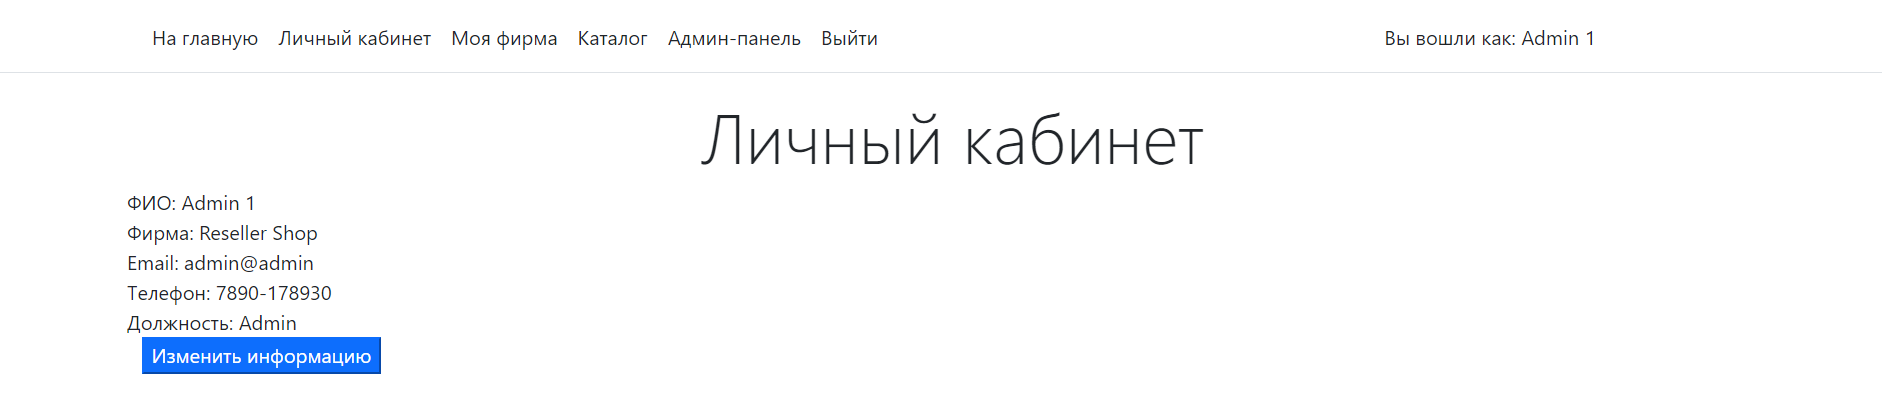
\includegraphics[width=\textwidth]{work_lk.png}}
	\caption{Личный кабинет}
	\label{work_lk}
\end{figure}

В кабинете фирмы выведена информация о фирме пользователя~(рис.~\ref{work_frm}).
По нажатию кнопки <<контракты>> открывается страница, на которой перечислины все контракты фирмы.
Также там расположена кнопка, открывающая форму добавления нового контракта (для менеджера).
У руководителя есть кнопка удаления контракта.
Можно перейти на страницу любого контракта: там выведена информация о нем и его содержимом, а также есть ссылка на его документ.
\begin{figure}[!h]
	\center{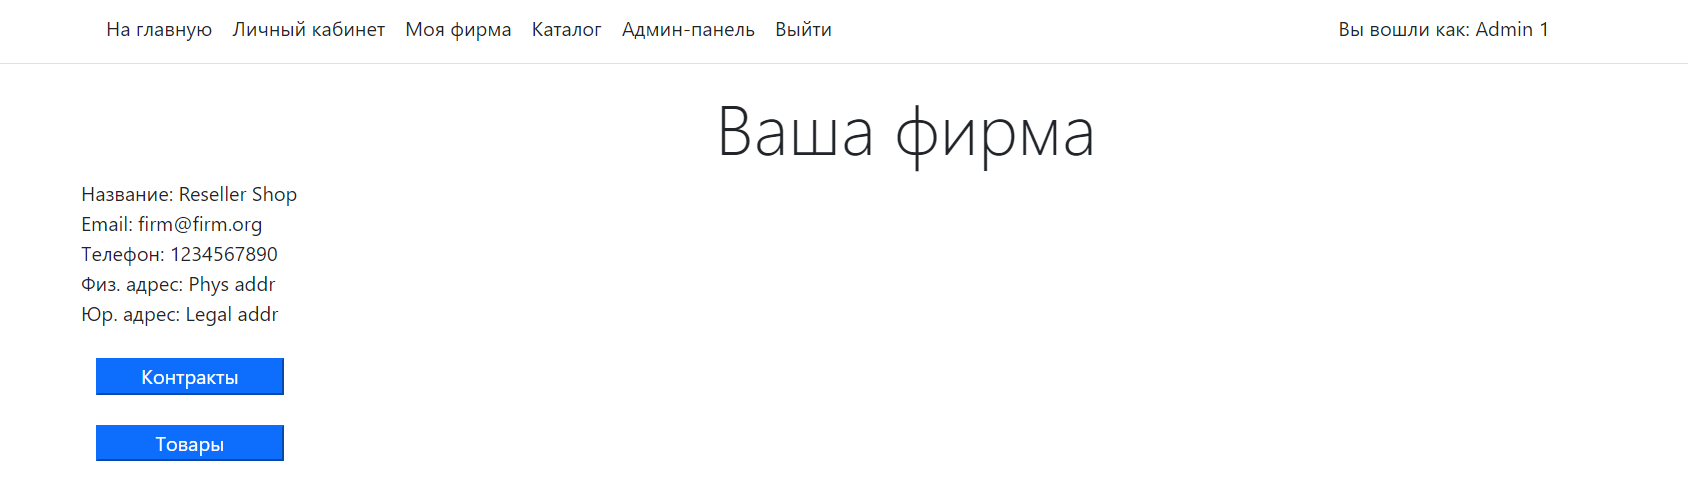
\includegraphics[width=\textwidth]{work_frm.png}}
	\caption{Кабинет фирмы}
	\label{work_frm}
\end{figure}

По нажатию кнопки <<товары>> открывается страница, на которой перечислины все товары фирмы.
Там же расположена кнопка, открывающая форму для добавления нового товара.
На страницу любого товара можно также перейти: там выведена информация о нем и складах, на которых он есть в наличии.
Существует возможность изменить или удалить товар, а также добавить его на склад.

В каталоге перечислены все товары, которые фирма пользователя может приобрести.
Есть возможность выбора категории товаров.

На странице аудита выводится список всех контрактов.
На страницу каждого контракта также можно войти: там перечислина вся информация о нем, а также есть ссылка на его документ.

В админ-панели можно получить доступ к управлению сущностями: категориями, производителями, пользователями, фирмами, товарами и складами (рис. \ref{work_ap}).
Есть страницы, на которых перечислены все сущности указанного типа, а также страницы каждой такой сущности.
Можно добавлять новые объекты, а также изменять или удалять существующие.
\begin{figure}[!h]
	\center{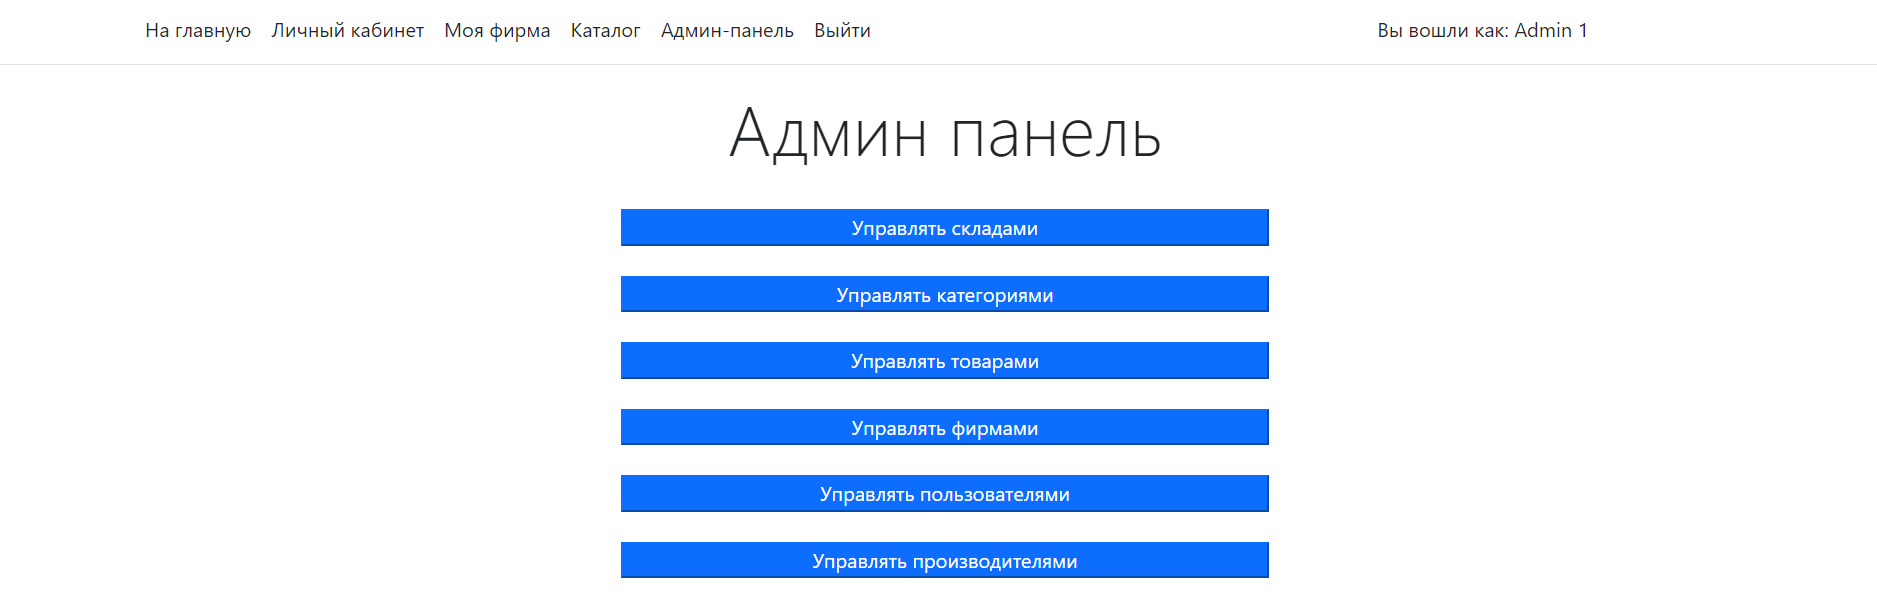
\includegraphics[width=\textwidth]{work_ap.png}}
	\caption{Админ-панель}
	\label{work_ap}
\end{figure}

\section{Тестирование}
Проведено модульное для компонента бизнес-логики и интеграционное тестирование для компонента доступа к данным.

В ходе модульного тестирования для каждого класса объекта модели тестируется:
\begin{itemize}
\item[---] добавление нового объекта;
\item[---] удаление объекта;
\item[---] получение объекта;
\item[---] изменение объекта;
\item[---] получение всех объектов объекта.
\end{itemize}

Для контракта тестируется также составление, подпись и получение всего содержимого контракта.

Для фирмы тестируется также получение всего штата сотрудников и получение всего списка товаров.

Для товаров тестируется получение всех товаров определенной категории.

В ходе модульного тестирования проведены следующие тесты:
\newpage
\begin{itemize}
	\item[---] добавление нового склада, его обновление и последующее удаление;
	\item[---] добавление нового товара, категории и производителя, их обновление и последующее удаление;
	\item[---] создание нового контракта, утверждение и подпись его с обеих сторон и последующее удаление;
\end{itemize}

Все тесты были пройдены успешно.

\section{Вывод из технологического раздела}
В данном разделе были приведены выбор средств реализации, реализация функции на стороне БД, реализация сущностей и ограничений целостности, описание интерфейса доступа к БД и описание тестов.